% ------------------------------------------------------------------------------
%
% PREAMBLE
%
% ------------------------------------------------------------------------------

\documentclass[12pt, titlepage]{article}


\usepackage{graphicx, amsmath, amssymb, natbib, setspace, sectsty, verbatim, 
		mathrsfs, float}
\usepackage{MnSymbol}
\usepackage{multirow}
\usepackage{bm}
\usepackage[usenames, dvipsnames]{color}
\bibpunct{(}{)}{;}{a}{}{,}
\setlength{\parindent}{3em}
%\parskip = 1.5ex
%\linespread{1.3}
%\onehalfspacing

\pdfpagewidth 8.5in
\pdfpageheight 11in
\setlength{\oddsidemargin}{0.0in} \setlength{\textwidth}{6.5in}
\setlength{\topmargin}{0.15in} \setlength{\textheight}{8.5in}
\setlength{\headheight}{0.0in} \setlength{\headsep}{0.0in}

\usepackage{/mnt/ExtraDrive1/Work/shTex/mymacros}

\providecommand{\norm}[1]{\lVert#1\rVert}
\newcommand{\csection}[1]{\section[#1]{\centering #1 }}
\subsectionfont{\small}
\newcommand{\cye}[1]{\color{yellow!70!black}#1}
\newcommand{\cre}[1]{\color{red!70!black}#1}
\newcommand{\cbl}[1]{\color{blue!70!black}#1}
\newcommand{\cgr}[1]{\color{green!70!black}#1}


% ------------------------------------------------------------------------------
%
% BEGIN DOCUMENT
%
% ------------------------------------------------------------------------------

\begin{document}

\setcounter{equation}{0}
\renewcommand{\theequation}{R.\arabic{equation}}


% ------------------------------------------------------------------------------
%
%                    Section 8.8.2
%                    Caribou forage data
%
% ------------------------------------------------------------------------------

{\large \flushleft \textbf{8.8.1 Caribou forage data}}

\vspace{.3cm}

Spatial models for the designed experiment using the caribou forage data (Figure 1.4) can be based on neighborhood relationships, which leads to linear models using spatial weights (Chapter 7), or, because the spatial arrangement is a grid pattern, distance among centriods is sensible, leading to geostatistical models (Chapter 6). We will investigate both approaches and compare them.

We fit models by maximizing the log-likelihood for a variety of models.  For spatial weights models, we defined neighbors based on ``rook's move,'' and denote that binary matrix as $\mathbf{W}_{1}$.  If this matrix was row-standardized, it is denoted $\overline{\mathbf{W}}_{1}$, with the corresponding diagonal matrix $\overline{\mathbf{K}}_{1}$.  If $\mathbf{W}_{1}$ is a symmetric spatial-weights matrix as described in Chapter 7, then a matrix that includes ``neighbors of neighbors'' is
$$
\mathbf{W}_{2} = \mathcal{I}(\mathcal{I}(\mathbf{W}_{1}\mathbf{W}_{1} > 0) + \mathbf{W}_{1} > 0) - \mathbf{I}
$$
where $\mathcal{I}(\cdot)$ is the indicator function, equal to 1 if its argument is true, otherwise it is zero, and $\mathbf{I}$ is the identity matrix to ensure that the diagonal of $\mathbf{W}_{2}$ is all zeros.  The corresponding diagonal matrix is denoted $\mathbf{K}_{2}$.  If $\mathbf{W}_{2}$ was row-standardized, it is denoted $\overline{\mathbf{W}}_{2}$, with the corresponding diagonal matrix $\overline{\mathbf{K}}_{2}$.

\begin{table}[H] 
	\caption{Model comparisons among a variety of covariance structures using MLE based on the minimized likelihood function ($-2L(\boldsymbol{\theta};\mathbf{y})$), AIC, BIC, and LOOCV.  The basic mean structure was $\boldsymbol{\mu} = \mu + \alpha_{i} + \gamma_{j} + \tau_{ij}$.  \label{tab:caribou_modcomp}}
\begin{center}
\begin{tabular}{|cc|crrr|}
  \hline
  \hline{}
  mean & $\boldsymbol{\Sigma}$ & $-2L(\boldsymbol{\theta};\mathbf{y})$ & AIC & BIC & LOOCV \\
	\hline
  \hline
	$\boldsymbol{\mu}$ & $\sigma^{2}\mathbf{I}$ & 
		-20.3 & -6.29 & 3.52 & 0.0465 \\ 
  $\boldsymbol{\mu}$ + row + col & $\sigma^{2}\mathbf{I}$ & 
		-42.9 & -10.92 & 11.50 & 0.0511 \\
  $\boldsymbol{\mu}$ & $\sigma^{2}(\mathbf{I} - \rho\mathbf{W}_{1})^{-1}\mathbf{K}_{1}$ & 
		-22.6 & -6.63 & 4.58 & 0.0396 \\
  $\boldsymbol{\mu}$ & $\sigma^{2}(\mathbf{I} - \rho\overline{\mathbf{W}}_{1})^{-1}\overline{\mathbf{K}}_{1}$ & 
		-24.7 & -8.69 & 2.52 & 0.0373 \\
  $\boldsymbol{\mu}$ & $\sigma^{2}(\mathbf{I} - \rho\mathbf{W}_{2})^{-1}\mathbf{K}_{2}$ &  -20.9 & -4.94 & 6.27 & 0.0396 \\ 
  $\boldsymbol{\mu}$ & $\sigma^{2}(\mathbf{I} - \rho\overline{\mathbf{W}}_{2})^{-1}\overline{\mathbf{K}}_{2}$ & 
		-23.1 & -7.14 & 4.07 & 0.0418 \\
  $\boldsymbol{\mu}$ & $\sigma^{2}(\mathbf{I} - \rho\mathbf{W}_{1})^{-1}(\mathbf{I} - \rho\mathbf{W}_{1}^{T})^{-1}$ & 
		-22.8 & -6.84 & 4.37 & 0.0394 \\ 
  $\boldsymbol{\mu}$ & $\sigma^{2}(\mathbf{I} - \rho\overline{\mathbf{W}}_{1})^{-1}(\mathbf{I} - \rho\overline{\mathbf{W}}_{1}^{T})^{-1}$ & 
		-24.0 & -8.02 & 3.19 & 0.0370 \\ 
  $\boldsymbol{\mu}$ & $\sigma^{2}(\mathbf{I} - \rho\mathbf{W}_{2})^{-1}(\mathbf{I} - \rho\mathbf{W}_{2}^{T})^{-1}$ & 
		-20.9 & -4.88 & 6.33 & 0.0394 \\
  $\boldsymbol{\mu}$ & $\sigma^{2}(\mathbf{I} - \rho\overline{\mathbf{W}}_{2})^{-1}(\mathbf{I} - \rho\overline{\mathbf{W}}_{2}^{T})^{-1}$ & 
		-21.0 & -4.99 & 6.22 & 0.0430 \\  
  $\boldsymbol{\mu}$ & $\sigma^{2}\textrm{sph}(\mathbf{D};\rho) + \delta^{2}\mathbf{I}$ & -22.7 & -4.69 & 7.92 & 0.0381 \\
  $\boldsymbol{\mu}$ & $\sigma^{2}\exp(-\mathbf{D}/\rho) + \delta^{2}\mathbf{I}$ & 
		-23.3 & -5.30 & 7.31 & 0.0389 \\
  \hline
  \hline
\end{tabular}
\end{center}
$\textrm{sph}(\mathbf{D};\rho) = (\mathbf{I} - 1.5\mathbf{D}/\rho + 0.5\mathbf{D}^{3}/\rho^{3})\mathcal{I}(\mathbf{D} < \rho)$
\end{table}

In Section 4.5.2 we examined two classical analyses of this designed experiment with uncorrelated errors, one where the two treatments, water and tarps, comprised the mean effects, and another with the same mean effects, but that also included row and column effects to account for spatial trends, at the expense of 9 more parameters.  Here, in Table~\ref{tab:caribou_modcomp}, we include those two models, along with a variety of CAR and SAR models with first and second-order neighbors, with and without row standardization, and the spherical and exponential geostatistical models. Table~\ref{tab:caribou_modcomp} shows $-2L(\boldsymbol{\theta};\mathbf{y})$, AIC, BIC, and LOOCV for model comparison.  While it may seem strange to include a metric of predictive performance, LOOCV is a valuable model diagnostic even when interest is centered on fixed effects because it evaluates the fit of both the mean structure and covariance structure.

\begin{figure}[H]
  \begin{center}
	    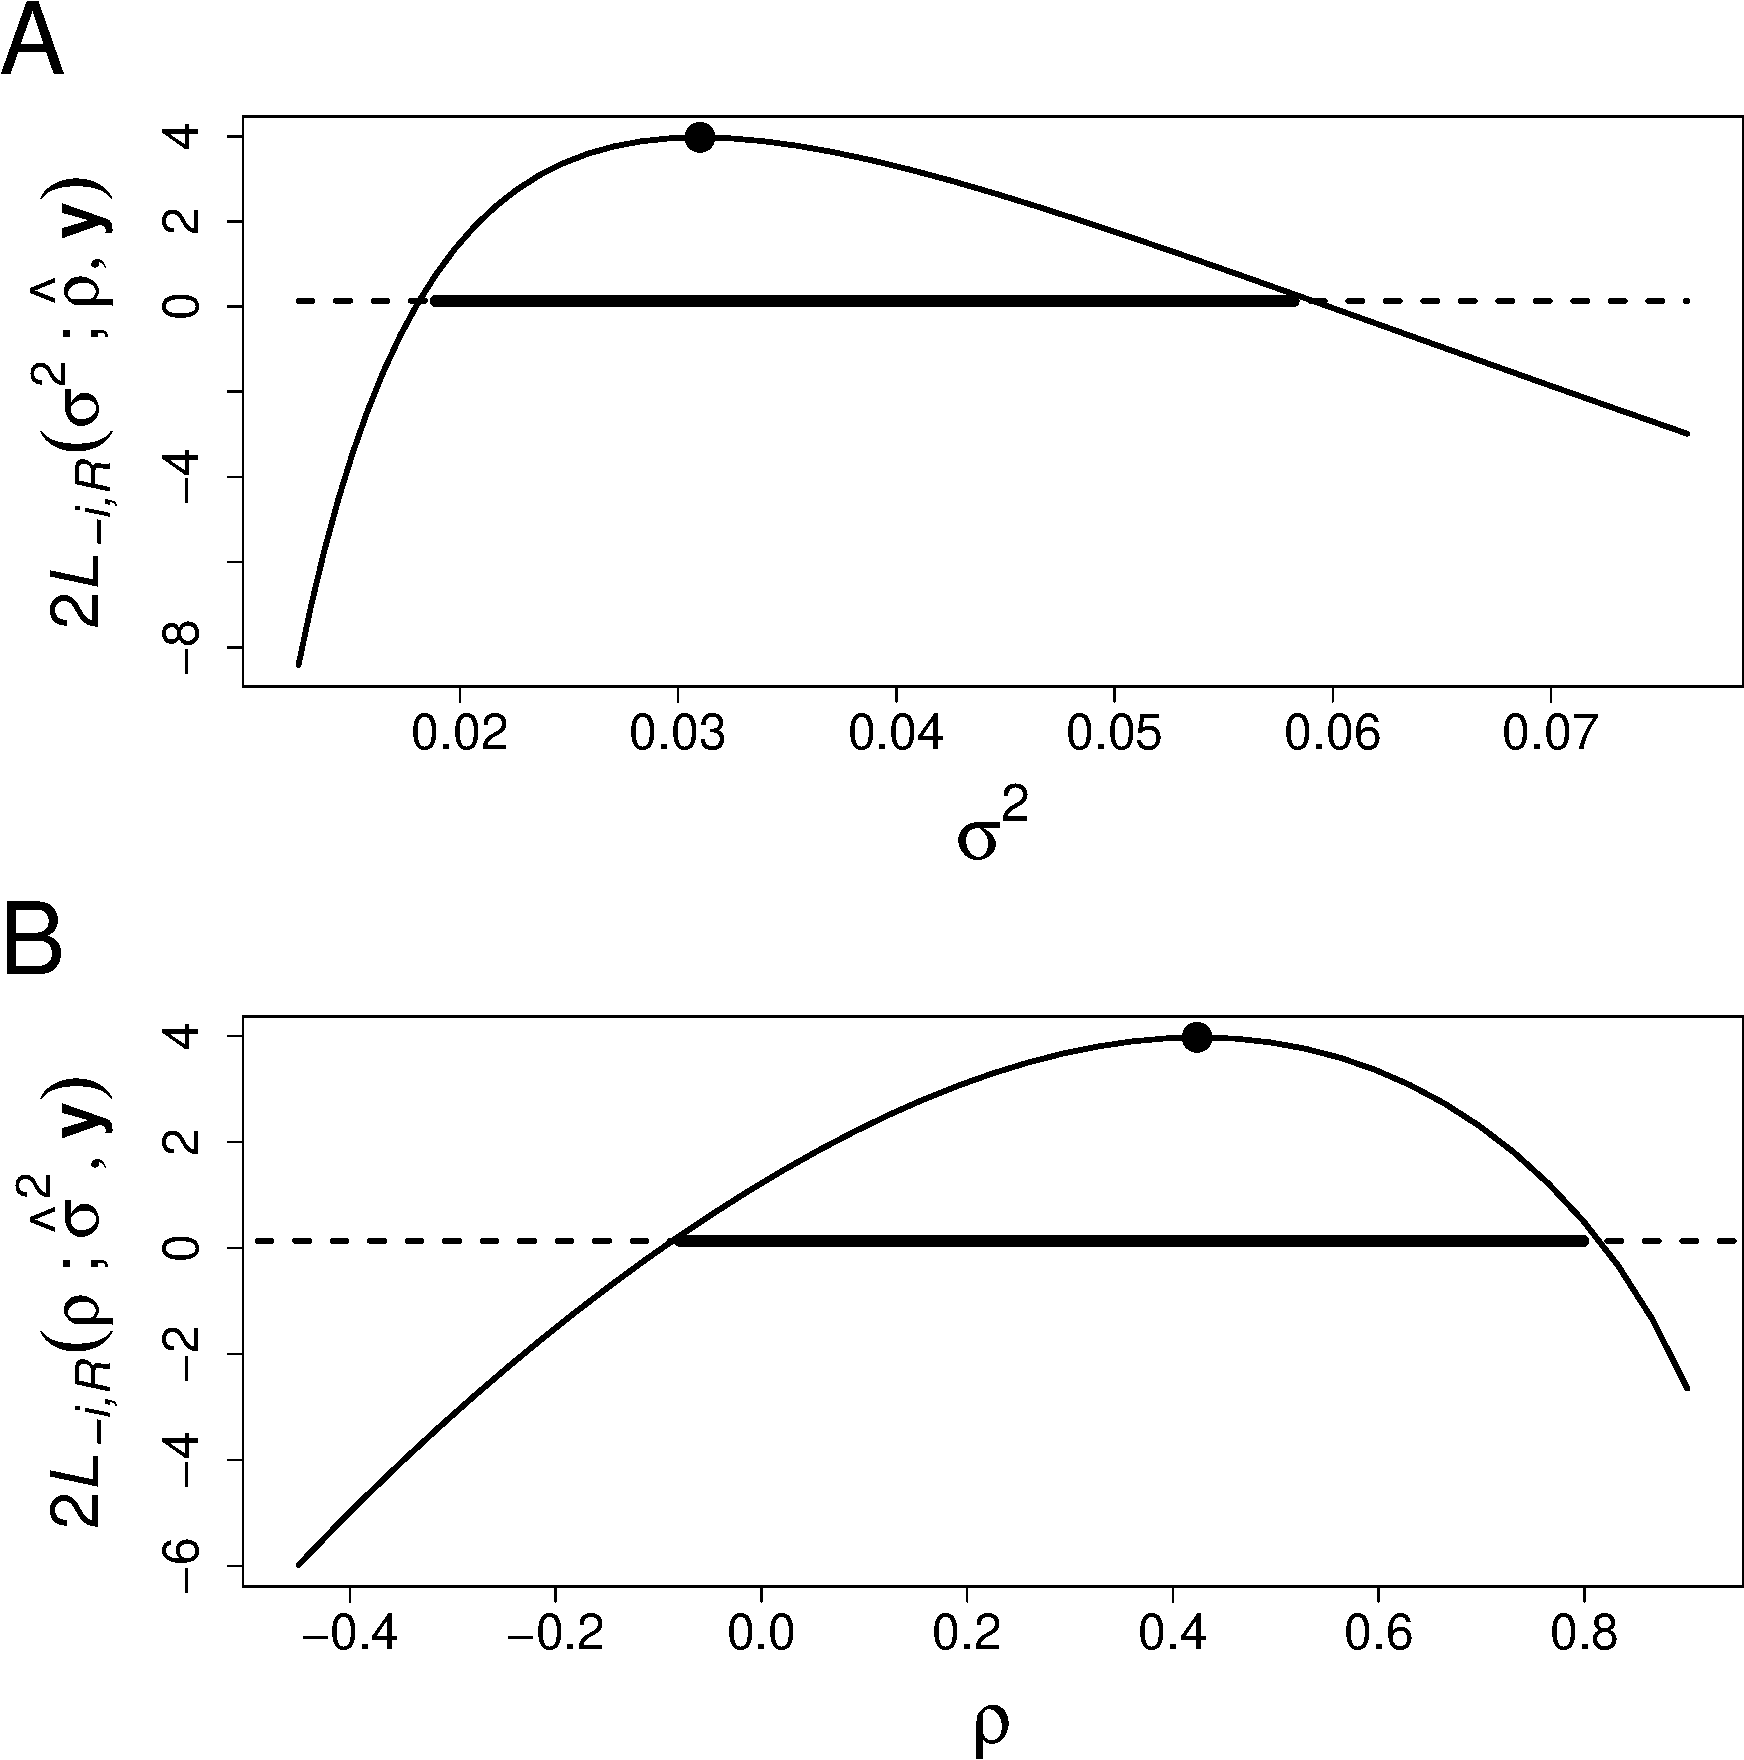
\includegraphics[width=.6\linewidth]{Caribou_proflike}
  \end{center}
  \caption{A. Profile likelihood confidence interval for $\sigma^{2}$ using REMLE. The curve is 2 times the restricted log-likelihood optimized for all parameters except $\sigma^{2}$, which is held constant at the value given by the x-axis.  The solid black circle is the REMLE, $\hat{\sigma}^{2}$, and the dashed line is $\hat{\sigma}^{2} - \chi^{2}(1-\alpha,1)$ for $\alpha = 0.05$.  The horizontal black line forms the 95\% confidence interval.  B. Profile likelihood confidence interval for $\rho$ in the same way as described above.  \label{Fig:Caribou_proflike}}
\end{figure}

Table~\ref{tab:caribou_modcomp} shows that the uncorrelated-error model with row and column effects minimizes $-2L(\boldsymbol{\theta};\mathbf{y})$ by a large margin among all models, but at the cost of 15 fixed effect parameters.  Even when penalizing for the extra fixed effects, AIC suggests that this is the best model, but it compared poorly to all other models based on BIC and LOOCV.  Among the spatial weights models, the first-order neighbor models with row standardization were best according to all 3 criteria, with little difference between CAR and SAR.  These two spatial weights models appear to be slightly better than both of the geostatistical models based on all 3 criteria.

\begin{figure}[H]
  \begin{center}
	    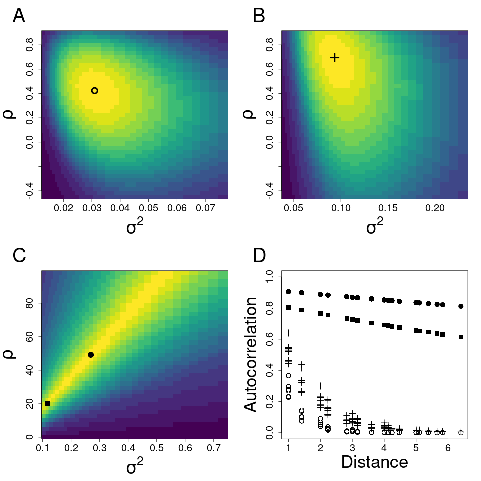
\includegraphics[width=.8\linewidth]{Caribou_compmod}
  \end{center}
  \caption{REML surfaces for caribou data where the mean model contains main effects and interaction between the water and tarp effects. A. Row-standardized, first-order SAR covariance structure, the open circle shows the REMLE. B. Row-standardized, first-order CAR covariance structure, the plus symbol shows the REMLE. C. Geostastitical-exponential covariance structure, where the solid circle shows the REMLE, and the solid square shows the REMLE with $\rho$ fixed at 20.  D. Autocorrelation as a function of distance between centroids, where the symbols correspond to each of the models in A, B, and C. \label{Fig:Caribou_compmod}}
\end{figure}

Based on the the results in Table~\ref{tab:caribou_modcomp}, we shall proceed with the row-standardized SAR model as the best model (as we already examined a CAR model for the example based on seal data).  As for the seal data, we used profile likelihood (Figure~\ref{Fig:Caribou_proflike}) to make inference about the covariance parameters. The REML estimate for $\rho$ was 0.424 with a 95\% confidence interval from -0.079 to 0.799, and the REMLE for $\sigma^{2}$ was 0.0310 with a 95\% confidence interval from 0.0189 to 0.0582.



Before making further inferences on the mean effects, we compare the REML surfaces among row-standardized, first-order CAR and SAR models and an exponential geostatistical model, where Figure~\ref{Fig:Caribou_compmod}A corresponds to the likelihood surface that was used to construct likelihood profile confidence intervals in Figure~\ref{Fig:Caribou_proflike}.  The row-standardized, first-order CAR model (Figure~\ref{Fig:Caribou_compmod}B) had $\hat{\rho} = 0.695$ and $\hat{\sigma}^{2} = 0.0934$, both substantially larger than the SAR model.  The resulting autocorrelation, plotted for all possible pairwise distances in Figure~\ref{Fig:Caribou_compmod}D, shows that, indeed, the CAR model has higher autocorrelation than the SAR model, and that both are non-stationary.  The geostastistical exponential model had a nugget effect of 0.0222, with a partial sill of 0.269 and a range of 49.2. We also held the range to 20, and then the REMLE for the nugget effect was 0.0218 with a partial sill of 0.118.  Part of the reason to hold the range at twenty was to observe how the likelihood is still optimized along the ridge of higher values, and to see how that affects our parameter estimates.  The resulting autocorrelation, plotted for all possible pairwise distances in Figure~\ref{Fig:Caribou_compmod}D, shows that both exponential models have stationary autocorrelation that is much higher than SAR and CAR models, and the model with range 49.2 is higher than the one with range 20.

\begin{table}[H] 
	\caption{Estimates are in the left 4 columns after the effect, and standard errors are the right 4 columns.  Effects are $\mu$ = intercept, $\alpha_{2}$ = watered, $\gamma_{2}$ = no tarp, $\gamma_{3}$ = shade tarp, $\tau_{22}$ = watered with no tarp, and $\tau_{23}$ = watered with shade tarp .  Fitted models are classical linear model with uncorrelated errors (LM), CAR and SAR models using $\overline{\mathbf{W}}_{1}$, and exponential geostatistical model (EXP), where EXP$^{*}$ has the range parameter fixed at 20. \label{tab:caribou_estse}}
\begin{center}
\begin{tabular}{|c|rrrrr|rrrrr|}
  \hline
  \hline{}
   & \multicolumn{5}{|c|}{Estimate} & \multicolumn{5}{c|}{Standard Error} \\
Effect & LM & SAR & CAR & EXP & EXP$^{*}$ & LM & SAR & CAR & EXP & EXP$^{*}$ \\
  \hline
  \hline{}
$\mu$ & 1.906 & 1.917 & 1.903 & 1.992 & 1.988 & 0.077 & 0.086 & 0.086 & 0.506 & 0.323 \\ 
$\alpha_{2}$ &  0.074 & 0.057 & 0.030 & 0.048 & 0.047 & 0.109 & 0.104 & 0.102 & 0.104 & 0.104 \\ 
$\gamma_{2}$ &   0.112 & 0.143 & 0.137 & 0.173 & 0.173 & 0.109 & 0.099 & 0.100 & 0.107 & 0.106 \\ 
$\gamma_{3}$ &   0.352 & 0.361 & 0.374 & 0.396 & 0.396 & 0.109 & 0.098 & 0.098 & 0.105 & 0.105 \\ 
$\tau_{22}$ &   -0.124 & -0.175 & -0.136 & -0.185 & -0.185 & 0.154 & 0.136 & 0.137 & 0.148 & 0.148 \\ 
$\tau_{25}$ &   -0.203 & -0.226 & -0.209 & -0.218 & -0.218 & 0.154 & 0.139 & 0.138 & 0.145 & 0.144 \\ 
  \hline
  \hline
\end{tabular}
\end{center}
\end{table}

Using the models in Figure~\ref{Fig:Caribou_compmod}, along with the classical uncorrelated model, Table~\ref{tab:caribou_estse} shows the estimated fixed effects, and their standard errors, using REMLE, recalling the model from Section 4.5.2, based on the constraints $\alpha_{1} = \gamma_{1} = 0$, $\tau_{1j} = 0$ for all $j$ and $\tau_{i1} = 0$ for all $i$.  Notice that the estimates change very little among models (Table~\ref{tab:caribou_estse}).  In fact, the standard errors are also quite consistent across models, except for the intercept effect, where there are large differences in the standard errors, especially for the exponential geostatistical models, compared to the uncorrelated and CAR and SAR models.  What is happening here?  First, notice that $\mu$ is a \textit{mean effect}, whereas all other effects are \textit{contrasts}.  That is, $\mu$ is the estimated nitrogen content for an unwatered plot with a clear tarp.  Every other effect in the table is an estimated deviation from $\mu$.  The effect $\alpha_{2}$ is the difference between watered and unwatered plots, etc.  It appears that when estimating the difference between effects, all models give very similar results, however when estimating a mean, there are substantial differences among model standard errors.  Is this generally true?  It is left as an exercise to use \texttt{spmodel} to consider the $2 \times 3$ combinations of water and tarp effects as a single effect with 6 levels, and estimate their means and standard errors without an overall intercept.

\begin{figure}[H]
  \begin{center}
	    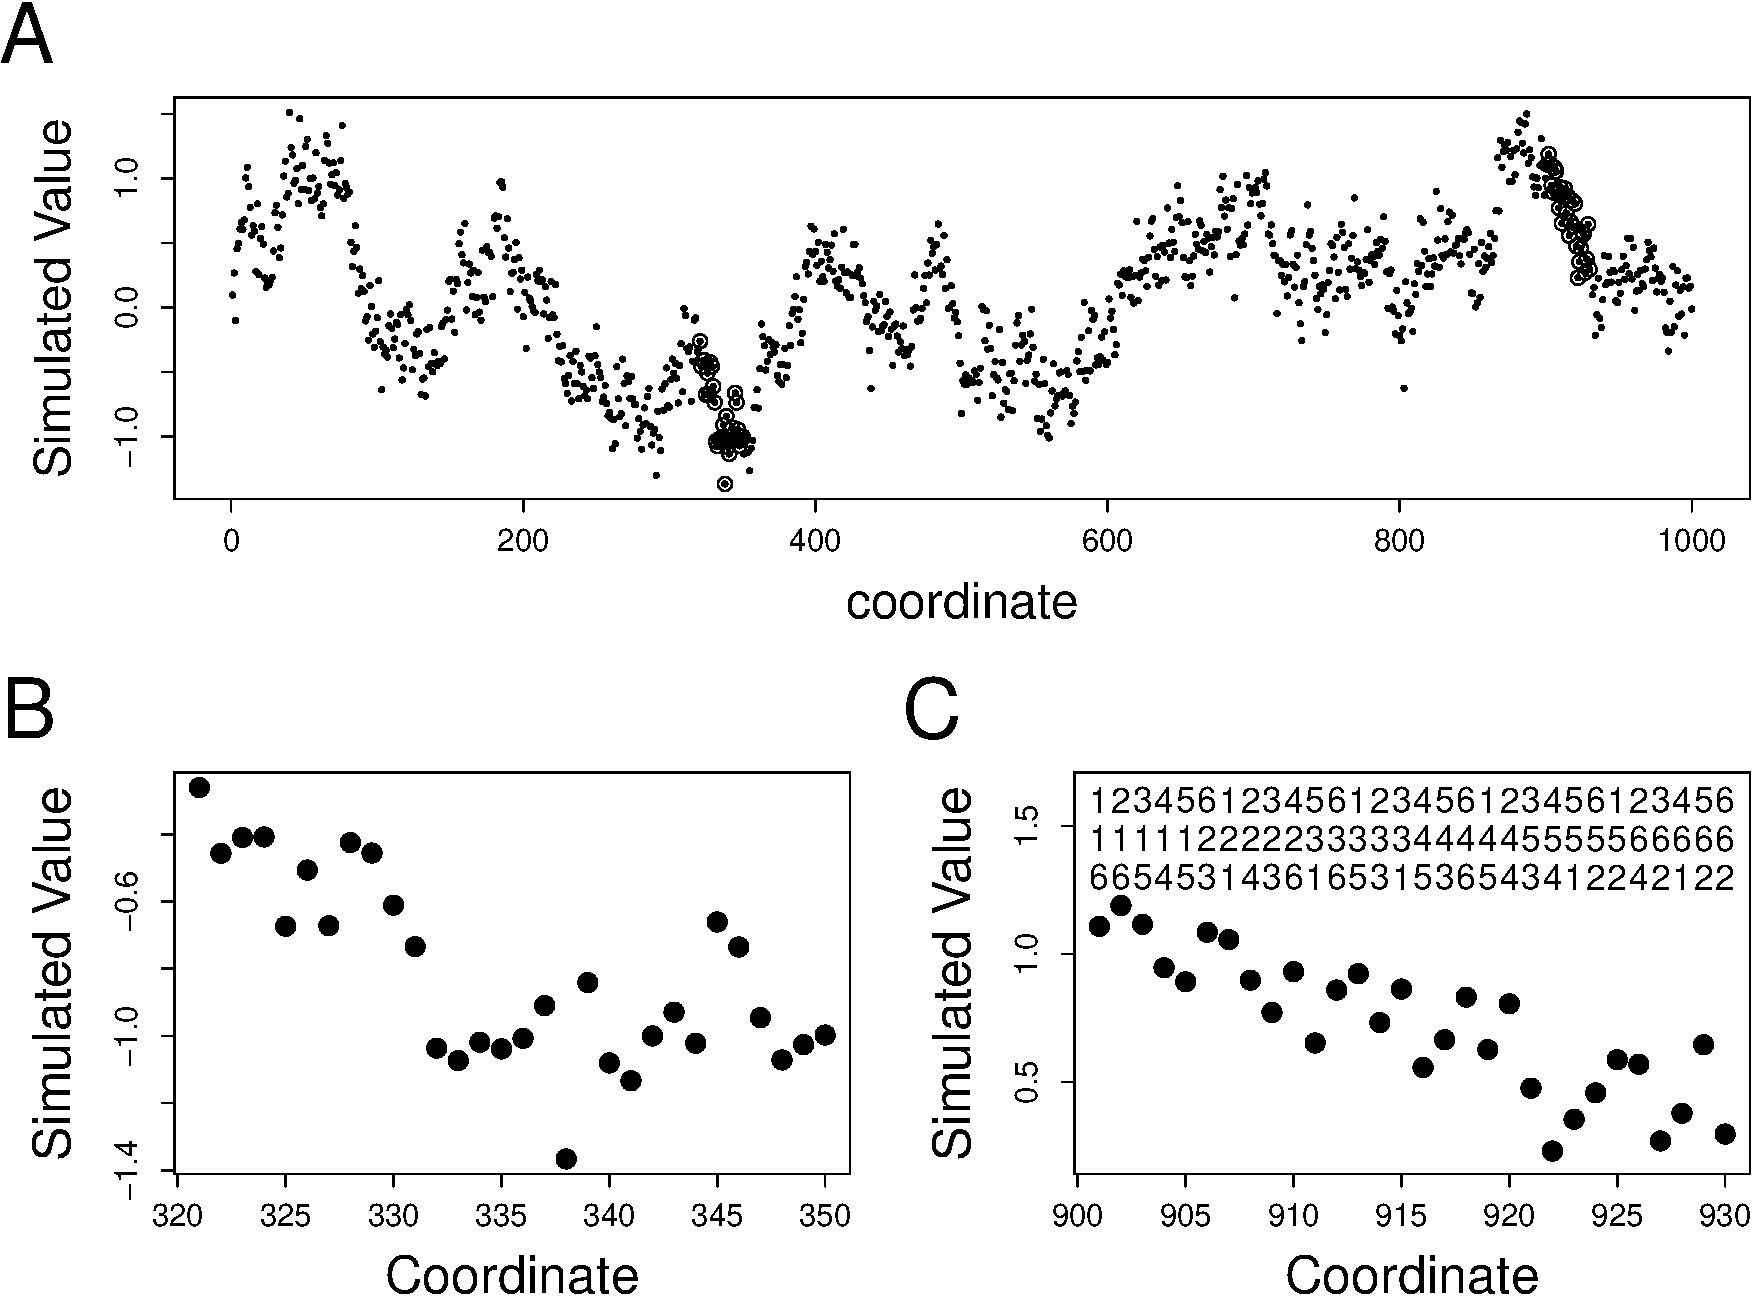
\includegraphics[width=.8\linewidth]{Caribou_sim1000}
  \end{center}
  \caption{A. 1000 values simulated from an exponential geostatistical model. B. A close-up of simulated values from locations 321 to 350.  C. A close-up of simulated values between 901 to 930.  The numbers above the simulated values are treatments labels; the top row is design 1, the middle row is design 2, and the bottom row is a randomized design. \label{Fig:Caribou_sim1000}}
\end{figure}

To examine further, let us consider the general idea of estimating the mean for autocorrelated data.  We simulated random variables on the integers from 1 to 1000 with a mean of zero using the exponential autocovariance model with a range of 49.2, a nugget of 0.0222, and a partial sill of 0.269 as estimated for the caribou forage data and shown in Figure~\ref{Fig:Caribou_compmod}. The simulated data are shown in Figure~\ref{Fig:Caribou_sim1000}A.  We added open circles around the values to highlight those simulated between coordinates 321 to 350, and between coordinates 901 to 930, which are shown in more detail in Figures~\ref{Fig:Caribou_sim1000}B,C. Notice that in both Figures~\ref{Fig:Caribou_sim1000}B,C, neither set of data contains the true mean zero, and there is a downward trend in both data sets.  In Figure~\ref{Fig:Caribou_sim1000}B, the trend is away from the mean, and in Figure~\ref{Fig:Caribou_sim1000}C, it is back towards the mean.  What this example illustrates is that autocorrelated data can ``wander'' away from the mean for long stretches, and the higher the autocorrelation, the farther it can wander from the mean.  Hence, when a model is fit to the data, and there is a high amount of autocorrelation, there will be a lot of uncertainty in estimating the mean.  In looking at Figures~\ref{Fig:Caribou_sim1000}B,C, without knowledge of the true values, how can one tell if the data are straddling the mean, wandering away from the mean, or wandering back towards the mean?  This uncertaintly can be seen in Table~\ref{tab:caribou_estse}, where models with increasing amounts of autocorrelation, as seen in Figure~\ref{Fig:Caribou_compmod}D, have higher standard errors for the intercept. 

How is it, then, that the models with spatial autocorrelation can estimate a contrast as well as, or even better than, the model with uncorrelated errors?  When considering models with an overall intercept, call it $\mu$, and the case of a single factor model with treatment effects $\alpha_{i}$, say, then an estimate of that treatment effect is $\mu + \alpha_{i}$.  A contrast between two treatment effects, say treatments 1 and 2, is $(\mu + \alpha_{1}) - (\mu + \alpha_{1}) = \alpha_{1} - \alpha_{2}$, and hence the uncertainty of estimating the overall mean is eliminated. By way of example, we took the data in Figure~\ref{Fig:Caribou_sim1000}C, and created an experiment with a single factor with 6 treatment levels and 3 different designs.  In design 1, we apply the treatments 1 through 6, in order, and repeat 5 times until all treatments have been applied to the 30 simulated values (top set of numbers over the data in Figure~\ref{Fig:Caribou_sim1000}C).  In design 2, we apply treatment 1 to the first 5 samples, treatment 2 to the second 5 samples, etc., until all treatments have been applied to the 30 simulated values (middle set of numbers over the data in Figure~\ref{Fig:Caribou_sim1000}C). In design 3, we apply treatments at random (bottom set of numbers over the data in Figure~\ref{Fig:Caribou_sim1000}C).  We set all 6 treatments to zero, and estimated treatments and contrasts.  We will concentrate on contrasts between treatments 1 and 2, $\ell_{1} = (1, -1, 0, 0, 0, 0)$, between 1 and 4, $\ell_{2} = (1, 0, 0, -1, 0, 0)$, and between 1 and 6, $\ell_{3} = (1, 0, 0, 0, 0, -1)$.  Because we have simulated the data and prescribed the treatments, we know the true values and can evaluate how a spatial model and uncorrelated model behave.  For the spatial model, we will also use the true covariance parameters that were used to simulate the data (exponential autocovariance model with a range of 49.2, a nugget of 0.0222, and a partial sill of 0.269), so we eliminate the issue of estimating those among the different designs.

The results are given in Table~\ref{tab:sim_estse}.  First, let us compare the estimates of all $\alpha_{i}$ between the uncorrelated model and the autocorrelated model for the randomized design.  For the uncorrelated model, each treatment estimate is simply the mean of the experimental units that received that treatment.  However, for the autocorrelated model, estimates are influenced by neighboring values.  If the neighboring values are above their treatment estimate, then the treatment estimate of a single experimental unit will be adjusted upward to allow the residuals to be autocorrelated (if positively autocorrelated, as we have here).  The sum effect of these adjustments is that the estimates for the autocorrelated model have much less variation, ranging from 0.692 to 0.836, while for the uncorrelated model they range from 0.452 to 0.984, and even the ranking of the means are different.  Recall that the true mean of these treatments is zero (zero was the mean of the simulated data, and all treatment effects were zero).  The uncorrelated model has a treatment estimate, $\alpha_{2}$, closest to the true mean, but it also has a treatment estimate, $\alpha_{6}$, farthest from the true mean, so is the uncorrelated model doing better or worse than the autocorrelated model?  Under squared error loss, the mean-squared error for the uncorrelated model is 

However, these data could have been produced by a process where the data straddled the true mean, in fact, suppose the true mean was the mean of the realized values in Figure~\ref{Fig:Caribou_sim1000}C, which was 0.726.  In this case, the spatial model would have better estimates under squared error loss; [(0.700 - 0.726)$^{2}$ +(0.716 - 0.726)$^{2}$ + $\ldots$ + (0.836 - 0.726)$^{2}$]/6 = 0.0024 versus [(0.661 - 0.726)$^{2}$ +(0.452 - 0.726)$^{2}$ + $\ldots$ + (0.984 - 0.726)$^{2}$]/6 = 0.0261.

The treatments were applied differently for designs 1 and 2, but they provide a useful comparison for the autocorrelated model. In design 2, the treatments are confounded with the trend, where $\alpha_{1}$ was applied to the values on the left of Figure~\ref{Fig:Caribou_sim1000}C, and $\alpha_{6}$ was applied to the values on the right of Figure~\ref{Fig:Caribou_sim1000}C.  This confounding shows up in the estimates, which range from 1.063 for $\alpha_{1}$ to 0.407 for $\alpha_{6}$ (Table~\ref{tab:sim_estse}), while the more spatially-balanced treatments of design 1 have much less variation in treatment estimates.  As for the case in the paragraph above, in general the squared error loss will be smaller for the less variable estimates given by the spatially-balanced treatments.

\begin{table}[H] 
	\caption{Estimates for the simulated data are in the left 4 columns after the effect or contrast, and standard errors are the right 4 columns.  IND is a fitted model with independent (uncorrelated) errors, while EXP is a model where autocovariance parameters are held constant (range of 49.2, a nugget of 0.0222, and a partial sill of 0.269). Des1 is design 1, where treatment labels are given in the top set of numbers over the data in Figure~\ref{Fig:Caribou_sim1000}C.  Des2 is design 2, where treatment labels are given in the middle set of numbers over the data in Figure~\ref{Fig:Caribou_sim1000}C.  Rand is a randomized design, where treatment labels are given in the lower set of numbers over the data in Figure~\ref{Fig:Caribou_sim1000}C. \label{tab:sim_estse}}
\begin{center}
\begin{tabular}{|c|r|rrr|r|rrr|}
  \hline
  \hline{}
   & \multicolumn{4}{|c|}{Estimate} & \multicolumn{4}{c|}{Standard Error} \\
  \hline
   & \multicolumn{1}{|c|}{IND} & \multicolumn{3}{c|}{EXP autocorr} & \multicolumn{1}{|c|}{IND} & \multicolumn{3}{c|}{EXP autocorr}\\
Effect & \multicolumn{1}{|c|}{Rand} & \multicolumn{1}{c}{Des1} & \multicolumn{1}{c}{Des2} & \multicolumn{1}{c|}{Rand} & \multicolumn{1}{|c|}{Rand} & \multicolumn{1}{c}{Des1} & \multicolumn{1}{c}{Des2} & \multicolumn{1}{c|}{Rand} \\
  \hline
  \hline{}
$\alpha_{1}$ & 0.661 & 0.818 & 1.063 & 0.700 & 0.106 & 0.464 & 0.496 & 0.467 \\ 
$\alpha_{2}$ &  0.452 & 0.817 & 1.119 & 0.716 & 0.106 & 0.465 & 0.494 & 0.468 \\ 
$\alpha_{3}$ &  0.746 & 0.698 & 0.970 & 0.692 & 0.106 & 0.466 & 0.493 & 0.469 \\ 
$\alpha_{4}$ &  0.690 & 0.628 & 0.779 & 0.717 & 0.106 & 0.466 & 0.493 & 0.467 \\ 
$\alpha_{5}$ &  0.823 & 0.683 & 0.439 & 0.702 & 0.106 & 0.465 & 0.494 & 0.469 \\ 
$\alpha_{6}$ &  0.984 & 0.767 & 0.407 & 0.836 & 0.106 & 0.464 & 0.496 & 0.467 \\ 
  \hline
$\ell_{1}$ & 0.209 & 0.001 & -0.055 & -0.015 & 0.149 & 0.104 & 0.179 & 0.127 \\ 
$\ell_{2}$ & -0.029 & 0.190 & 0.285 & -0.016 & 0.149 & 0.112 & 0.295 & 0.109 \\ 
$\ell_{3}$ & -0.323 & 0.051 & 0.657 & -0.135 & 0.149 & 0.108 & 0.368 & 0.120 \\ 
  \hline
  \hline
\end{tabular}
\end{center}
\end{table}

Turning our attention to the standard errors, we see that, due to the balanced design, the standard errors for all uncorrelated models are equal at 0.106 (Table~\ref{tab:sim_estse}).  If we divide the smallest estimate, 0.452 by its standard error as an approximate z-test, we see that 0.452/0.106 = 4.264, which compared to 1.96 for an alpha-level test of 0.05, we would make the Type I error of falsely rejecting the null hypothesis that this treatment was zero.  In fact, Type I errors occur for all treatments under the uncorrelated model.  In contrast, the largest z-value for the autocorrelated model with the randomized design is 0.836/0.467 = 1.790, and as this is less than 1.96, we would not make the Type I error at alpha-level 0.05, nor would we for any of the other treatments.  Now we can see how the inflated variances of the autocorrelated model protect us against the Type I error as the model accounts for the data wandering away from the mean, depending on how much autocorrelation exists.

The same is true for design 1, the spatially-balanced design.  It is easy to verify, by similar calculations as given above, that no Type I errors occur at alpha-level 0.05.  However, the same is not true for design 2, the confounded design.  Here, we would make the Type I error for treatments $\alpha_{1}$, $\alpha_{2}$, and $\alpha_{3}$.  In fact, it even gets worse if we estimate the amount of autocorrelation, rather than holding the covariance parameters at their true values (exponential autocovariance model with a range of 49.2, a nugget of 0.0222, and a partial sill of 0.269).  The confounding of the mean essentially transfers spatial pattern from the errors to the mean structure, so that the estimated autocorrelation goes down, causing even further Type I errors.  It is left as an exercise for the reader to verify this.  Also, note that we have framed the too-small standard errors for the uncorrelated model, and the better standard errors for the autocorrelated model, in a hypothesis-testing framework.  One could form confidence intervals as an alternative framework, and then the uncorrelated model would not cover the true values, while the autocorrelated model would.

Next, we turn our attention to contrasts, $\ell_{1} - \ell_{3}$ in Table~\ref{tab:sim_estse}.  Recall that the true value for all contrasts is zero, and that, for the uncorrelated model, a z-value for $\ell_{3}$ is |-0.323|/0.149 = 2.168, which is greater then 1.96, so we would commit a Type I error at $\alpha = 0.05$.  Looking again at Figure~\ref{Fig:Caribou_sim1000}C, we can see why.  Notice that treatment 6 occurs mostly at the lower coordinates (left half), leading higher than average values.  Of course, this occured just by chance, and that is the nature of randomized designs, and 20\% of the time we should expect Type I errors.  Even though treatment 2 is not in any of our contrasts, note how it occurs at the higher coordinates (right half), and would also lead to Type I errors when contrasted with certain treatments, especially treatment 6.  Interestingly, for this design, the spatially autocorrelated model does not make the Type I error, even though it estimates a smaller standard error (0.120 for autocorrelated, versus 0.149 for uncorrelated).  As we discussed earlier, the autocorrelated model adjustments the treatment estimates so that there is much less variation than the uncorrelated model, and hence the contast is smaller, mitigating some of the unbalanced nature of the randomized design.  It is left as an exercise for the reader to see how bad the Type I error can be for the uncorrelated model for this particular randomized design by contrasting treatment 2 to treatment 6, and then see if the autocorrelated model also commits the Type I error.  It is the ability of the autocorrelated model to mitigate some unbalanced application of treatments by weighting data in ways other than simple means, and the fact that it is estimating a difference that eliminates the overall mean, that allows the autocorrelated model to have smaller standard errors than the uncorrelated model when estimating a contrast, even for randomized designs.

In comparing design 1 versus design 2 for the autocorrelated model in Table~\ref{tab:sim_estse}, the balanced nature of design 1 keeps all three contrasts near zero, while design 2 estimates a large difference for $\ell_{3}$ because treatments 1 and 6 are at opposite ends of the trending data.  However, this is appropriately reflected in the standard errors, as those for design 2 are much larger than those for design 1.  Interestingly, even for the extreme constast $\ell_{3}$ under design 2, the z-value is 0.567/0.368 = 1.54, so no Type I error would be committed.  It is very clear from this example, though, that the spatially-balanced application of treatments is a much better design than the spatial clustering of treatments, and also that the spatially-balanced design is much better than a randomized design as judged by the standard errors.

We conclude this rather long digression by reducing this notion of estimating means versus contrasts with a very simple example to further explain the differences.  Let us suppose that we have two random variables, $\varepsilon_{1}$ and $\varepsilon_{2}$, with mean zero, unit variance, and correlation between them equal to $0 \le \rho \le 1$.  Then if we add the same treatment to both $\varepsilon_{1}$ and $\varepsilon_{2}$, and use the mean to estimate the treatment effect, then the variance of that mean will be $(2 + 2\rho)/2^{2}$.  If $\rho = 0$, then we obtain the familiar variance of a mean assuming independence, $\sigma^{2}/n$, which in this case is $1/2$.  On the other hand, the worst case scenario is when $\rho = 1$, in which case the variance is 1.  In is easy to extend this idea to more than 2 random variables, where the variance under zero correlation is $1/n$ for $n$ random variables, while the variance for correlation 1 (among all pairwise random variables) remains 1.  Thus, as sample size increases, the uncorrelated model is much, much better than maximum correlation.  

Now, consider adding treatment 1 to $\varepsilon_{1}$ and treatment 2 to $\varepsilon_{2}$ and estimating their difference.  In this case, the variance of that difference will be $(2 - 2\rho)$.  When the correlation is zero, the variance is 2, but as $\rho \rightarrow 0$, the variance goes to zero.  What this means, practically, is that when treatments are side by side in a designed experiment where there is a high amount of positive spatial autocorrelation, the variance between them is smaller than if there was no autocorrelation, and better than if they were farther apart in the experimental design.  We can see this in design 1 for $\ell_{1}$, where treatment 1 is always next to treatment 2, while in design 1, treatment 1 is never next to treatment 4, so the variance of $\ell_{2}$ is higher than $\ell_{1}$.  Design 1 also has treatment 1 next to treatment 6, except for the very first and last plots, so the variance of $\ell_{3}$ is larger than that of $\ell_{1}$.  It is left as an exercise to find a better design than design 1 if one were only interested on contrasts between treatments 1 and 2, between 3 and 4, and between 5 and 6, and how much better it might be than design 1?

Finally, we turn our attention back to Table~\ref{tab:caribou_estse}, where all standard errors for contrasts are lower for the spatially-autocorrelated models than for the uncorrelated model, which makes sense according to our simulation, especially if the design has spatial balance.  In fact, looking again Figure 1.4, there is a certain symmetry in treatments.  If we flip the design upside down, top to bottom, the tarp treatments do not change, while the watered treatments change from Y to N and vice-versa.  This design was not random, but optimized for certain contrasts, which is explained more fully in Ver Hoef (2012).  For the harbor seal data, we showed how ANOVA tables and likelihood ratio tests could be applied to the data after fitting a spatial model, and that could be done here, too.  

However, here we focus on the use of planned contrasts, as in Ver Hoef (2012), where there were 16 such contrasts, and one can proceed directly to estimating those contrasts once the spatial model has been fit.  For example, one of those contrasts was the main effect of shade tarp versus no tarp, and if the treatments were labeled $\tau_{1}$ to $\tau_{3}$ for shade, clear, and no tarps, respectively, for watered plots, and labeled $\tau_{4}$ to $\tau_{6}$ for shade, clear, and no tarps, respectively, for unwatered plots, then we were interested in contrast $\ell = (1, 0, -1, 1, 0, -1)$. For the SAR model using $\boldsymbol{\Sigma} = \sigma^{2}(\mathbf{I} - \rho\overline{\mathbf{W}}_{1})^{-1}(\mathbf{I} - \rho\overline{\mathbf{W}}_{1}^{T})^{-1}$, with $\hat{\sigma}^{2} = 0.0310$ and $\hat{\rho}^{2} = 0.424$, we obtain a contrast estimate of 0.385 with a standard error of 0.148, yielding a $z$-value of 2.608, which is considerably larger than the 1.96 cutoff value for an alpha-level test at $P = 05$.  More details on these data, and obtaining optimum designs, can be found in Ver Hoef (2012).







%%%%%%%%%%%%%%%%%%%%%%%%%%%%%%%%%%%%%%%%%%%%%%%%%%%%%%%%%%%%%%%%%%%%%%%%%%%%%%%%
%%%%%%%%%%%%%%%%%%%%%%%%%%%%%%%%%%%%%%%%%%%%%%%%%%%%%%%%%%%%%%%%%%%%%%%%%%%%%%%%                BIBLIOGRAPHY
%%%%%%%%%%%%%%%%%%%%%%%%%%%%%%%%%%%%%%%%%%%%%%%%%%%%%%%%%%%%%%%%%%%%%%%%%%%%%%%%
%%%%%%%%%%%%%%%%%%%%%%%%%%%%%%%%%%%%%%%%%%%%%%%%%%%%%%%%%%%%%%%%%%%%%%%%%%%%%%%%

%\bibliographystyle{consbiol}
\bibliographystyle{/mnt/ExtraDrive1/Work/shTex/asa}
\bibliography{DaleChap883.bib}
%\bibliographystyle{/home/jay/Data/shTex/shTex/asa}
%\bibliography{/home/jay/Data/shTex/shTex/StatBibTex.bib}




\end{document}

